\section{Misure preliminari}
\todo{inserire una introduzione} MAGARI ANCHE FOTO BOARD
\subsection{Segnale PPG}
Come descritto della sezione 2.1.0(\ref{cap:Hardware}), sono stati realizzati due differenti sistemi per l'acquisizione di segnali fotopletismografici e che ospitano due diversi moduli PPG. In questo studio l'obiettivo è quello dimostrare il funzionamento di questi sistemi, cioè che il segnale acquisito sia idoneo ad una successiva elaborazione e quindi stima dei parametri di interesse. Infatti, il segnale PPG puro non rappresenta una stima di alcun parametro, ma solo grazie ad una successiva elaborazione, tramite opportuni algoritmi, che è possibile ottenere la stima desiderata.
Tuttavia, anche dal segnale PPG puro è possibile fare alcune considerazioni sulla sua morfologia e sulle informazioni che contiene \cite{Foroozan2018}. In figura \ref{fig:Descrizione_Segnale_PPG} è possibile vedere un chiaro segnale PPG acquisito sulla parte superiore del polso e filtrato da rumore e disturbi esterni. Da questa immagine si può notare una certa periodicità del segnale che corrisponde proprio al ritmo cardiaco.
\begin{figure}[h]
	\centering
	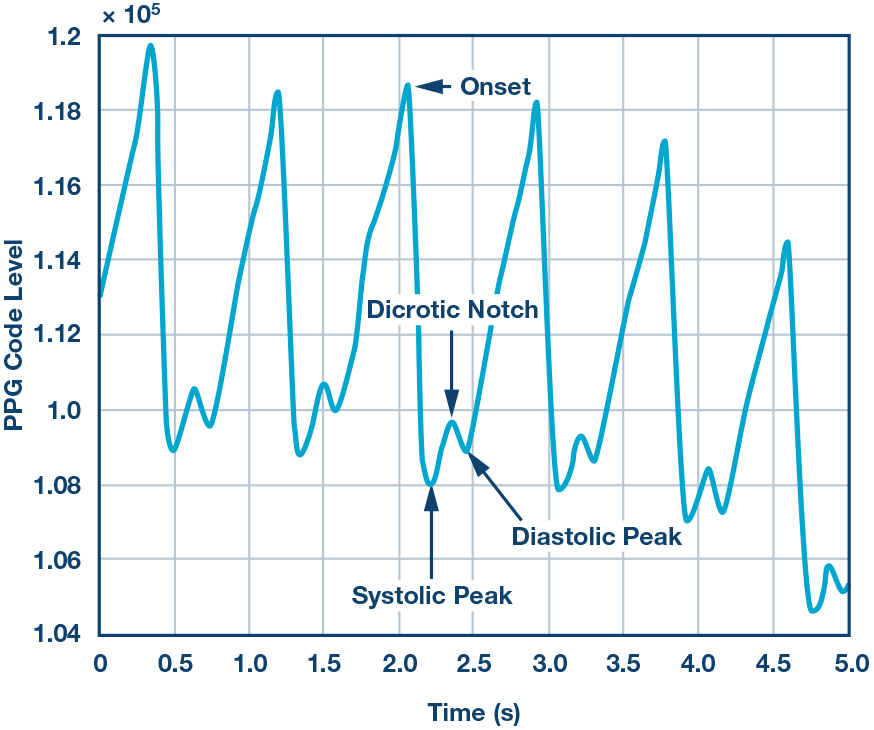
\includegraphics[width=0.8\linewidth]{ImageFiles/Misure Preliminari/descrizione_segnale_ppg}
	\caption{Segnale PPG acquisito sul polso (immagine tratta da Foroozan \cite{Foroozan2018}).}
	\label{fig:Descrizione_Segnale_PPG}
\end{figure}
Oltre alla periodicità, è presente anche una forte similarità tra la morfologia del segnale PPG e la forma d'onda della pressione arteriosa. Infatti, come si può vedere sempre in figura \ref{fig:Descrizione_Segnale_PPG}, è possibile identificare due minimi separati da un massimo locale che corrispondono a dei punti caratteristici della pressione arteriosa. In particolare, il primo minimo(quello più piccolo) corrisponde al picco sistolico, il secondo minimo invece indica il picco diastolico mentre il massimo locale che li separa rappresenta la tacca dicrotica. \todo{non so se andare nel dettglio del significato medico}
L'esempio di segnale fotopletismografico riportato non è quello che viene acquisito, ma una sua elaborazione volta a rimuovere i disturbi. Infatti, il segnale PPG è molto suscettibile a diversi sorgenti di disturbo tra cui la scarsa perfusione sanguigna, gli artefatti dovuti al movimento e l'illuminazione dell'ambiente circostante. Per limitare questi disturbi viene fatto un primo passaggio di filtraggio del segnale PPG acquisito in modo da renderlo pronto per l'estrazione effettiva della stima desiderata. In alcuni casi questo può avvenire con l'ausilio di altri dispositivi, oltre al sensore PPG, come avviene nei sistemi progettati in questo studio dove si utilizza un accelerometro triassiale per la stima degli artefatti dovuti al movimento e quindi per compensare i disturbi introdotti, da questo fenomeno, nel segnale PPG misurato.

\subsection{Misurazioni preliminari sui soggetti}
\todo{inserire proceduradi acquisizione }


\paragraph{Configurazione dei moduli PPG}~

\noindent \\ I moduli PPG MAX86916 e MAXM86161, impiegati nelle board progettate, permettono di effettuare diverse configurazioni che dipendono dalla specifica applicazione e dalle stime di interesse dal momento che il segnale PPG, come evidenziato nella sezione precedente, contiene diverse informazioni che devono essere estratte con opportuni algoritmi. Di seguito vengono riportate le configurazioni utilizzate per effettuare delle misure preliminari, atte a verificare l'efficacia delle schede realizzate.

\paragraph{Adapater Board: MAXM86161}
\todo{la facciamo appena abbiamo le medie}
\paragraph{Adapater Board: MAX86916}
Per l'\textit{Adapeter Board} che monta il sensore MAX86916 è stata scelta la configurazione riportata in tabella \ref{tab:ConfigMAX86916}:
\begin{table}[h]
	\renewcommand{\arraystretch}{1.5}
	\centering
	\footnotesize
	\begin{tabular}{cccc}
		\textbf{Numero di campioni mediati} & 1 \\ \hline
		\textbf{Frequenza di acquisizione [Hz]} & 100 \\ \hline
		\textbf{Fondo scala ADC [nA]} & 16384 \\ \hline
		\textbf{Corrente di alimentazione dei LED [mA]} & 2.0 \\ \hline
		\textbf{Larghezza impulso luce LED [$\mu$s]} & 420 \\ \hline
		\textbf{Modalità operativa} & FLEX MODE \\ \hline
	\end{tabular}
	\caption{Confronto delle caratteristiche degli accelerometri.}
	\label{tab:ConfigMAX86916}
\end{table}
\todo{Da commentare i parametri scelti}



\todo{misure}
\todo{commenti}